\section{110 --- Balanced Binary Tree}
Given a binary tree, determine if it is height-balanced.

For this problem, a height-balanced binary tree is defined as: 

\begin{quote}
a binary tree in which the depth of the two subtrees of every node never differ by more than 1.
\end{quote}

\paragraph{Example 1:}
\begin{flushleft}
\textbf{Input}: \fcj{[3,9,20,null,null,15,7]}

\begin{figure}[H]
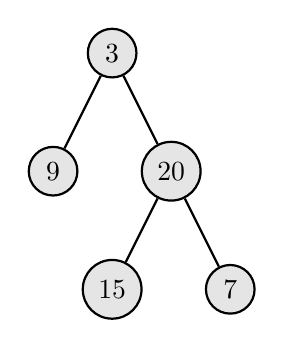
\begin{tikzpicture}
[every node/.style={draw, circle, fill=gray!20!, minimum size=5mm},
%level 1/.style={sibling distance=25mm},
%level 2/.style={sibling distance=15mm},
thick]
\node{3}
child{node{9}}
child{node{20} child{node{15}} child{node{7}}};
\end{tikzpicture}
\end{figure}

\textbf{Output}: \fcj{true}
\end{flushleft}
\paragraph{Example 2:} 
\begin{flushleft}
\textbf{Input}: \fcj{[1,2,2,3,3,null,null,4,4]}
\begin{figure}[H]
\begin{tikzpicture}
[mynode/.style={draw,circle,minimum size=5mm, fill=gray!20!}]
\node(){};
\node[mynode](1) {1};
\node[mynode](2l) [below = 8mm of 1, xshift=-6mm] {2};
\node[mynode](2r) [below = 8mm of 1, xshift=6mm] {2};
\node[mynode](3l) [below = 8mm of 2l, xshift=-6mm] {3};
\node[mynode](3r) [below = 8mm of 2l, xshift=6mm] {3};
\node[mynode](4l) [below = 8mm of 3l, xshift=-6mm] {4};
\node[mynode](4r) [below = 8mm of 3l, xshift=6mm] {4};
\draw[>=stealth,->] (1) -- (2l);
\draw[>=stealth,->] (1) -- (2r);
\draw[>=stealth,->] (2l) -- (3l);
\draw[>=stealth,->] (2l) -- (3r);
\draw[>=stealth,->] (3l) -- (4l);
\draw[>=stealth,->] (3l) -- (4r);
\end{tikzpicture}
\end{figure}

\textbf{Output}: \fcj{false}

 \end{flushleft}
 \subsection{Recursion}
根据题目中的定义,高度平衡二叉树是每一个结点的两个子树的深度差不能超过1,那么肯定需要一个求各个点深度的函数,然后对每个节点的两个子树来比较深度差,但是这种方法效率差,因为每一个点都会被上面的点计算深度时访问一次,优化后的方法是如果我们发现子树不平衡,则不计算具体的深度,而是直接返回-1。那么优化后的方法为:对于每一个节点,递归获得左右子树的深度,如果子树是平衡的,则返回真实的深度,若不平衡,直接返回$-1$
%\setcounter{algorithm}{0}
%\begin{algorithm}[H]
%\caption{Recursion}
%\begin{algorithmic}[1]
%\Procedure{IsBalanced}{$T$}
%\If{$\texttt{MaxDepth} < 0$}
%\State \Return \texttt{false}
%\EndIf
%\State \Return \texttt{true}
%\EndProcedure
%\end{algorithmic}
%\end{algorithm}
%\texttt{MaxDepth} 在计算每个节点的最大深度时,同时进行左右子树深度的比较,如果深度大于1,返回$-1$,否则返回实际的最大深度。
%\begin{algorithm}[H]
%\caption{Include Balance Check In Computing Maximum Depth}
%\begin{algorithmic}[1]
%\Function{MaxDepth}{$T$}
%\If{$T=\texttt{null}$}
%\State \Return 0
%\EndIf
%\State $\alpha:=\texttt{MaxDepth}(\texttt{LEFT}(T))$ \Comment The maximum depth of left subtree
%\If{$\alpha < 0$} \Comment Left subtree is unbalanced
%\State \Return $-1$
%\EndIf
%\State $\beta:=\texttt{MaxDepth}(\texttt{RIGHT}(T))$ \Comment The maximum depth of right subtree
%\If{$\beta < 0$} \Comment Left subtree is unbalanced
%\State \Return $-1$
%\EndIf
%\State $d:=|\alpha-\beta|$ \Comment The absolute difference
%\If{$d > 1$}
%\State \Return $-1$ \Comment $T$ is unbalanced
%\EndIf
%\State \Return $1+\max(l, r)$ \Comment $T$ is balanced so return the actual maximum depth
%\algstore{110algo}
%\end{algorithmic}
%\end{algorithm}
%\begin{algorithm}[H]
%\begin{algorithmic}[1]
%\algrestore{110algo}
%\EndFunction
%\end{algorithmic}
%\end{algorithm}